%%
%
% ARQUIVO: main.tex
%
% VERSÃO: 1.0
% DATA: Maio de 2016
% AUTOR: Coordenação de Trabalhos Especiais SE/8
% 
%  Arquivo tex principal do documento de Projeto de Fim de Curso (PFC).
%  Este arquivo SÓ PRECISA SER MODIFICADO NA PARTE DE CONTEÚDO:
%
%    a. colocar um \include{•} para cada capítulo do documento de PFC.
%
%%

% -----
% CLASSE DO DOCUMENTO DE PFC
% -----
\documentclass{pfc}

% -----
% PACOTES LATEX USADOS NO DOCUMENTO DE PFC
% -----
\usepackage[brazilian]{babel}
\usepackage[utf8]{inputenc}
\usepackage[T1]{fontenc}

\usepackage{amsmath}
\usepackage{graphicx}
\usepackage{tabularx}
\usepackage{float}
\usepackage{color}
\usepackage{amsfonts,amssymb}
\usepackage[authoryear]{natbib}

\usepackage{enumitem}
\usepackage{rotating}
\usepackage{lipsum}
\usepackage{lastpage}
\usepackage{stringstrings}
\usepackage{pgffor}
\usepackage{pdftexcmds}

% -----
% MARGENS DO DOCUMENTO DE PFC
% -----
\usepackage{geometry}
\geometry{
	a4paper,
	total={210mm,297mm},
	left=25mm,
	right=25mm,
	top=25mm,
	bottom=30mm,
	textwidth=160mm,
	textheight=242mm,
	headheight=0mm,
	headsep=0mm,
}

% -----
% DECLARAÇÕES AUXILIARES PARA REFERÊNCIAS
%
%  Diferencia \citet e \citep de acordo com a NBR 10520:2002
% -----
\DeclareRobustCommand{\NATand}{;}
\DeclareRobustCommand{\NATetal}{et~al.}
\makeatletter
\renewcommand{\NAT@nmfmt}[1]{%
  \ifNAT@swa\expandafter\MakeUppercase
  \else\DeclareRobustCommand{\NATand}{ e}\expandafter\@firstofone\fi{{\NAT@up #1}}%
}
\makeatother

% -----
% AMBIENTE DE FIGURAS DE PFC
%
%  A classe do documento está configurada SOMENTE para figuras no formato EPS.
%  Logo, use PREFERENCIALMENTE este tipo de arquivo.
%
%    a. os arquivos das figuras devem estar no diretório 'img'
% -----
\graphicspath{{./img/}}

% -----
% INÍCIO DO DOCUMENTO DE PFC
% -----
\begin{document}

% -----
% PARTE PRÉ-TEXTUAL DE PFC
%
% Alterar o CONTEÚDO dos arquivos siglas.tex E pre-texto.tex
% -----
%%
%
% ARQUIVO: dados-pfc.tex
%
% VERSÃO: 1.0
% DATA: Maio de 2016
% AUTOR: Coordenação de Trabalhos Especiais SE/8
% 
%  Arquivo tex com os dados acerca do documento de PFC e da apresentação.
%
%   nos campos que definem nomes (autor; orientador; co-orientador; membros da banca)
%   É PRECISO usar os COMANDOS LaTeX para acentuação, conforme abaixo:
%
%         \'a - á || \`a - à || \~a - ã || \^a - â 
%         \'e - é || \^e - ê || \'i - í 
%         \'o - ó || \~o - õ || \^o - ô 
%         \'u - ú || \"u - ü
%
%%

%%% AUTORES DO PFC (Nome completo)
% ---
%  aceita até 03 autores (de autorI até autorIII)
%    a. preencher sucessivamente a partir de autorI
%    b. REMOVER as definições não necessárias
% ---
\autorI{Pedro Igor de Ara\'ujo Oliveira}
\autorII{Bruno Vieira Costa}
\autorIII{Lucas Ricarte Rogério Teixeira}

%%% POSTOS DOS AUTORES DO PFC
% ---
%  aceita os postos de até 03 autores (de postoautorI até postoautorIII)
%    a. preencher sucessivamente a partir de postoautorI (que deve ser o posto de autorI)
%    b. se o autorX É CIVIL, NÃO DEFINIR postoautorX (remover a linha de definição)
%    c. se o autorX É MILITAR, DEFINIR postoautorX com UMA das seguintes ALTERNATIVAS: Alu / 1 Ten / Cap
% ---
\postoautorI{1 Ten}

%%% TITULO DO PFC
\titulo{Ferramentas de classificação multidimensional para plataforma de auxílio ao aprendizado}

%%% DATA DA APRESENTAÇÃO (formato {dd}{Mmmmm}{aaaa})
\datadefesa{14}{Maio}{2018}

%%% ORIENTADOR DO PFC
% ---
%  CAMPO 1: P (para Prof.); PA (para Profa.); ou qualquer coisa (inclusive VAZIO) - o que for escrito aparecerá no documento
%  CAMPO 2: Nome completo
%  CAMPO 3: D (para D.Sc.); P (para Ph.D.); M (para M.Sc.) ou qualquer coisa (inclusive VAZIO) - o que for escrito aparecerá no documento
%  CAMPO 4: Instituição (com "do / da")
% ---
\orientador{P}{Alex de Vasconcellos Garcia}{D}{do IME}

%%% CO-ORIENTADOR DO PFC
% ---
%  se não houver co-orientador, REMOVA ESTA LINHA
%  preenchimento idêntico a \orientador{}{}{}{}
% ---
% \coorientador{P}{Nome Completo do Co-orientador}{P}{do IME}

%%% NÚMERO DA ENTRADA DA BIBLIOTECA (pegar na Biblioteca do IME)
\biblioref{004.69}{S586e}

%%% PALAVRAS-CHAVES DO PFC
% ---
%  devem ser separadas por vírgula e É OBRIGATÓRIO ter pelo menos uma
% ---
\palavraschaves{Classificação de texto, Processamento de linguagem natural, Ferramenta de auxílio ao aprendizado, Aprendizado de máquina}

%%% OUTROS MEMBROS DA BANCA DO PFC
% ---
%  aceita até mais 05 membros (de membrobancaI até membrobancaV)
%    a. preencher sucessivamente a partir de membrobancaI
%    b. REMOVER as definições não necessárias
%
%  cada membro tem preenchimento idêntico a \orientador{}{}{}{}
% ---
\membrobancaI{P}{Ronaldo Ribeiro Goldschmidt}{D}{da PUC-RJ}
\membrobancaII{P}{Julio Cesar Duarte}{D}{da PUC-RJ}
%\membrobancaIII{}{Nome do Membro da Banca 3}{}{da COPPE/UFRJ}
%\membrobancaIV{}{Nome do Membro da Banca 4}{}{da UNIRIO}
%\membrobancaV{}{Nome do Membro da Banca 5}{}{da UERJ}

%%
%
% ARQUIVO: pre-texto.tex
%
% VERSÃO: 1.0
% DATA: Maio de 2016
% AUTOR: Coordenação de Trabalhos Especiais SE/8
% 
%  Arquivo tex para a criação da parte pré-textual do documento de Projeto de Fim de Curso.
%
%%


% -----
% PÁGINA DE CAPA DO DOCUMENTO DE PFC
% -----
\makecapa

% -----
% PÁGINA DE TÍTULO DO PFC
% -----
\prepareadvisors
\maketitle

% -----
% PÁGINA DE CRÉDITOS DO DOCUMENTO DE PFC
% -----
\makecredits

% -----
% PÁGINA DE FOLHA DE ASSINATURAS
% -----
\preparemembers
\approvalpage

% -----
% PÁGINA DE DEDICATÓRIA (OPCIONAL, ie. pode remover toda a página)
% -----
%%% DEDICATÓRIA - PREENCHER...
% \dedicatoria{%
% Ao Instituto Militar de Engenharia, alicerce da minha formação e aperfeiçoamento.
% }%
% \makededication

% -----
% PÁGINA DE AGRADECIMENTOS (OPCIONAL, ie. pode remover toda a página)
% -----
%%% AGRADECIMENTOS - PREENCHER...
\agradecimentos{%
Agradecemos a todas as pessoas que nos incentivaram, apoiaram e possibilitaram esta oportunidade de ampliar nossos horizontes. \\
\indent
Em especial ao Professor Orientador Dr. Alex Garcia.
}%
\makethanks

% -----
% PÁGINA DE EPÍGRAFE (OPCIONAL, ie. pode remover toda a página)
% -----
%%% EPÍGRAFE - PREENCHER...
\epigrafe{%
Not everything that can be counted counts; and not everything that counts can be counted.}%
\autorepigrafe{%    %% Se não tem autor, coloque "Anônimo"
Anônimo
}%
\makeepigraph

% -----
% PÁGINA DE SUMÁRIO
% -----
\tableofcontents

% -----
% PÁGINAS DE LISTAS DE FIGURAS E DE TABELAS
% se a Dissertação não possui figuras e/ou tabelas, REMOVA O COMANDO CORRESPONDENTE
% -----
\listoffigures
\listoftables

% -----
% PÁGINA DE LISTA DE SIGLAS
% se a Dissertação não possui siglas, REMOVA TODA A PÁGINA
% -----
%%% SIGLAS - PREENCHER...
\acronimo{API}{\textit{Application programming interface}}
\acronimo{AWS}{\textit{Amazon Web Services}}
\acronimo{CNN}{\textit{Convolutional Neural Network}}
\acronimo{CPU}{\textit{Central processing unit}}
\acronimo{EAD}{Ensino à distância}
\acronimo{GPU}{\textit{Graphics Processing Unit }}
\acronimo{HTML}{\textit{Hypertext Markup Language}}
\acronimo{HTTP}{\textit{Hypertext Transfer Protocol}}
\acronimo{IA}{Inteligência Artificial}
\acronimo{JSON}{\textit{JavaScript Object Notation}}
\acronimo{LSTM}{\textit{Long Short Term Memory}}
\acronimo{NB}{\textit{Naive Bayes}}
\acronimo{NN}{\textit{Neural Network}}
\acronimo{RNN}{\textit{Recurrent Neural Network}}
\acronimo{SepCNN}{\textit{Separable Depthwise Convolutional Neural Network}}
\acronimo{SVM}{\textit{Support Vector Machine}}
\acronimo{TF-IDF}{\textit{Term Frequency-Inverse Document Frequency}}
\acronimo{VM}{\textit{Virtual Machine}}
\listofnicks

% -----
% PÁGINA DE LISTA DE ABREVIATURAS
% se a Dissertação não possui abreviaturas ou símbolos, REMOVA TODA A PÁGINA
% -----
%%% ABREVIATURAS - PREENCHER...
%\abreviatura{Ja}{jacobiano}
%\abreviatura{JS}{fluxo secundário (difusivo)}
%\abreviatura{M}{número de Mach}
%
%%%% SÍMBOLOS - PREENCHER...
%\simbolo{$\Phi$}{termo de dissipação viscosa}
%\simbolo{$\Gamma$}{coeficiente de difusão efetivo}
%\simbolo{$\alpha$}{fator de sub-relaxação}
%\simbolo{$\phi$}{variável dependente da equação diferencial geral}

%\listofsymbols

% -----
% PÁGINA DE RESUMO
% -----
%%% RESUMO - PREENCHER...
\resumo{%
Ferramentas de auxílio ao aprendizado são usadas nas mais diversas etapas da educação formal ou informal. Estas ferramentas costumam empregar diversas tecnologias. Dentre elas, pode-se incluir a classificação de documentos, pois essas plataformas são, em geral, grandes agregadoras de conteúdo de ensino. Para uma melhor acessibilidade de todo esse conteúdo, é necessário que ele seja categorizado, o que nem sempre é viável de ser realizado manualmente devido ao grande volume e a necessidade de conhecimento técnico sobre os assuntos abordados. Nesse contexto, pode ser aplicada a Classificação Automática de Documentos.\\
\indent
Este trabalho tem como objetivo analisar e implementar modelos consagrados de classificação de texto, aplicando-os para a classificação de enunciados de questões em avaliações de ensino segundo seus assuntos. A partir da exploração dessas técnicas, desenvolveu-se um modelo híbrido de classificador especializado em enunciados de questões.}%
\makeresumo

% -----
% PÁGINA DE ABSTRACT
% -----
%%% ABSTRACT - PREENCHER...
\abstract{%
Learning aid tools are used in the most diverse stages of formal or informal education. These tools usually employ various technologies. Among them, one can include the classification of documents, since these platforms are, in general, great aggregators of teaching content. For a better accessibility of all this content, it needs to be categorized, which is not always feasible to be done manually due to the large volume and the need for technical knowledge on the issues addressed. In this context, it's interesting to apply the Automatic Document Classification.\\
\indent
This work aims to analyze and implement established text classification models, applying them to the classification of question statements in teaching assessments according to their subjects. From the exploration of these techniques, a hybrid classifier model was developed that specializes in question statements.
}%
\makeabstract

\parindent 0.75cm

% -----
% PARTE DE CONTEÚDO DE PFC
%
%  Escrever cada capitulo do documento de PFC em um arquivo .tex separado.
%  Adicionar os arquivos .tex ao documento com comando \include{•}
% -----
%%
%
% ARQUIVO: cap-01.tex
%
% VERSÃO: 1.0
% DATA: Maio de 2016
% AUTOR: Coordenação de Trabalhos Especiais SE/8
% 
%  Arquivo tex de exemplo de capítulo do documento de Projeto de Fim de Curso.
%
% ---
% DETALHES
%  a. todo capítulo deve começar com \chapter{•}
%  b. usar comando \noindent logo após \chapter{•}
%  c. citações para referências podem ser
%       i. \citet{•} para citações diretas (p. ex. 'Segundo Autor (2015)...'
%       ii. \citep{•} para citações indiretas (p. ex. '... (AUTOR, 2015)...'
%  d. notas de rodapé devem usar dois comandos
%       i. \footnotemark para indicar a marca da nota no texto
%       ii. \footnotetext{•}, na sequência, para indicar o texto da nota de rodapé
%  e. figuras devem seguir o exemplo
%       i. devem ficar no diretório /img e devem ser no formato EPS
%  f. tabelas devem seguir o exemplo
%  g. figuras e tabelas podem ser colocadas em orientação landscape
%       i. figuras: usar \begin{sidewaysfigure} ... \end{sidewaysfigure}
%                   em vez de \begin{figure} ... \end{figure}
%       ii. tabelas: usar \begin{sidewaystable} ... \end{sidewaystable}
%                    em vez de \begin{table} ... \end{table}
%  h. toda figura e tabela deve ser referenciada ao longo do texto com \ref{•}
% ---
%%

\chapter{Introdução}
\noindent
O objetivo deste trabalho é desenvolver um algoritmo que classifique uma questão inédita de concurso dentre um conjunto de assuntos pré-determinados. Para atingir este objetivo, serão exploradas técnicas de aprendizado de máquina e processamento de linguagem natural.


\section{Motivação}
%porque estudar o tema é importante/relevante?

\subsection{Plataformas de auxílio ao aprendizado}
Neste relatório, será entendido por PAA qualquer software que tenha objetivo pedagógico. Existe um mercado de educação à distância (EAD) que por seu caráter remoto, propicia o uso de tecnologia digital para a facilitação do ensino.  Esse mercado tem se tornado competitivo e ganhado cada vez mais importância.

\subsection{Classificação automática de assuntos}

Será entendido por CAA qualquer método de classificação de textos exequível via software sem auxílio de um operador. Os principais métodos existentes são listados na seção de Métodos.
A CAA já é amplamente utilizada na indústria, por exemplo, em sites de notícias, gerenciadores de emails ou motores de busca.

\subsection{Loona}
Loona é um motor de busca em desenvolvimento pela empresa PaperX. Trata-se de uma ferramenta de busca de vídeos por imagem.

\begin{figure}[!ht]
	\centering
	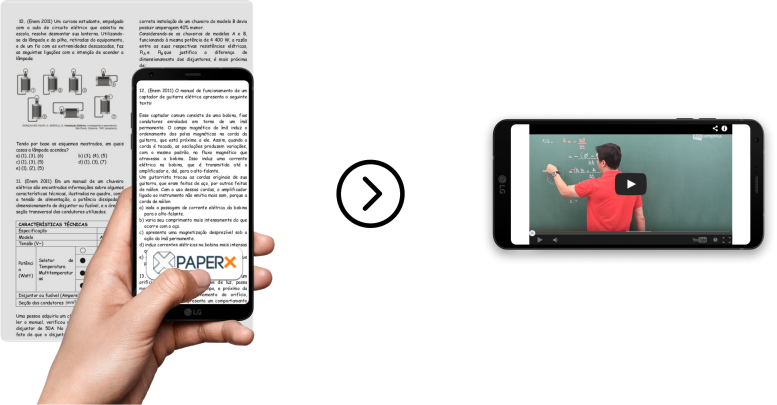
\includegraphics[width=0.4\textwidth]{figures/loona.png}   
	\caption{Funcionamento do loona}
	\label{fig:loona}
\end{figure}


\section{Objetivo}
%que tentará ser alcançado (principal e secundários)
O funcionamento do motor de busca em questão é dividido em três etapas:
\begin{itemize}
\item Reconhecimento ótico de caracteres (OCR); 
\item Classificação de texto e
\item Busca
\end{itemize}

\begin{figure}[!ht]
	\centering
	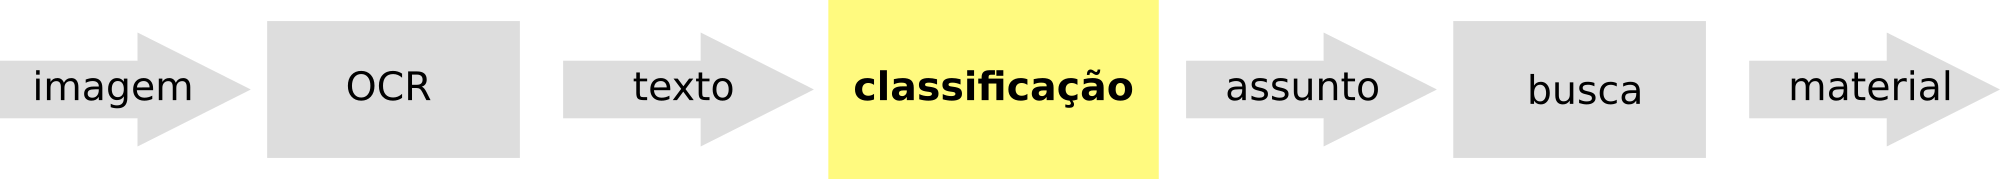
\includegraphics[width=0.4\textwidth]{figures/fluxograma.png}   
	\caption{Fluxo funcional da ferramenta}
	\label{fig:fluxograma}
\end{figure}


Este trabalho será restrito a etapa central: Classificação de texto.


% \section{Justificativa}
%a importância do trabalho no contexto institucional

\section{Metodologia}
%como o trabalho deverá ser conduzido
A primeira etapa do trabalho corresponde à obtenção de dados para serem utilizados nos algoritmos de aprendizado de máquina. Isso é feito a partir de Web scraping de questões de concursos públicos já rótuladas com os seus respectivos assuntos.

Em seguida, há uma fase de processamento de dados que remove inconsistências e prepara uma interface ideal para os algoritmos que serão aplicados posteriormente.

A terceira fase é a parte central do trabalho e consiste em explorar diferentes modelos para a classificação de questões. Cada um desses modelos possui suas particularidades com diferentes arquiteturas e hiperparâmetros para uma otimização de acordo com o contexto dos dados utilizados.

Como etapa final, a solução ótima encontrada de classificação é implementada na plataforma de auxílio ao aprendizado da paperx.com.br para o uso em ferramentas de busca.


\section{Estrutura}
%do documento
Sobre os capítulos subsequentes a seguinte distribuição de conteúdo:
\begin{itemize}
\item Capítulo 2: 
fundamentação teórica sobre cada um dos algoritmos de classificação que serão utilizados;
\item Capítulo 3:
descrição da implementação para cada uma das etapas descritas na metodologia;
\item Capítulo 4:
comparação dos resultados dos entre diferentes modelos implementados.
\end{itemize}

% -----
% PARTE DE REFERÊCIAS BIBLIOGRÁFICAS DE PFC
%
%  As referências do documento de PFC devem estar no arquivo refs.bib
%  Devem seguir o formato bibtex - ver Manual-Referencias.pdf para mais detalhes.
% -----
\bibliographystyle{pfc}
\bibliography{refs}

% -----
% PARTE DE APÊNDICE DE PFC
%
%  Se o documento de PFC não tiver apêndices REMOVER AS LINHAS ABAIXO
%  Adicionar os arquivos .tex de apêndice ao documento com comando \include{•}
% -----
\inappendix
%%
%
% ARQUIVO: apendice.tex
%
% VERSÃO: 1.0
% DATA: Maio de 2016
% AUTOR: Coordenação de Trabalhos Especiais SE/8
% 
%  Arquivo tex de exemplo de apêndice do documento de Projeto de Fim de Curso.
%  Este exemplo traz dois apêndices (dois comandos \chapter{•}). Poderiam ser colocados em arquivos .tex
%  separados. Neste caso, o arquivo main.tex deveria ter um \include{•} para cada arquivo .tex
%
% ---
% DETALHES
%  a. todo apêndice deve começar com \chapter{•}
%  b. usar comando \noindent logo após \chapter{•}
%  c. segue os mesmos DETALHES do arquivo .tex de exemplo de capítulo do documento de Projeto de Fim de Curso
% ---
%%
\chapter{Apêndice Exemplo}
\noindent
Curabitur tortor. Pellentesque nibh. Aenean quam. In scelerisque sem at dolor. Maecenas mattis. Sed convallis tristique sem. Proin ut ligula vel nunc egestas porttitor. Morbi lectus risus, iaculis vel, suscipit quis, luctus non, massa. Fusce ac turpis quis ligula lacinia aliquet. Mauris ipsum. Nulla metus metus, ullamcorper vel, tincidunt sed, euismod in, nibh. Quisque volutpat condimentum velit.

Class aptent taciti sociosqu ad litora torquent per conubia nostra, per inceptos himenaeos. Nam nec ante. Sed lacinia, urna non tincidunt mattis, tortor neque adipiscing diam, a cursus ipsum ante quis turpis. Nulla facilisi. Ut fringilla. Suspendisse potenti. Nunc feugiat mi a tellus consequat imperdiet. Vestibulum sapien. Proin quam. Etiam ultrices. Suspendisse in justo eu magna luctus suscipit. Sed lectus. Integer euismod lacus luctus magna.

Lorem ipsum dolor sit amet, consectetur adipiscing elit. Integer nec odio. Praesent libero. Sed cursus ante dapibus diam. Sed nisi. Nulla quis sem at nibh elementum imperdiet. Duis sagittis ipsum. Praesent mauris. Fusce nec tellus sed augue semper porta. Mauris massa. Vestibulum lacinia arcu eget nulla. Class aptent taciti sociosqu ad litora torquent per conubia nostra, per inceptos himenaeos. Curabitur sodales ligula in libero. Sed dignissim lacinia nunc.

\chapter{Apêndice Exemplo 02}
\noindent
Curabitur tortor. Pellentesque nibh. Aenean quam. In scelerisque sem at dolor. Maecenas mattis. Sed convallis tristique sem. Proin ut ligula vel nunc egestas porttitor. Morbi lectus risus, iaculis vel, suscipit quis, luctus non, massa. Fusce ac turpis quis ligula lacinia aliquet. Mauris ipsum. Nulla metus metus, ullamcorper vel, tincidunt sed, euismod in, nibh. Quisque volutpat condimentum velit.

Class aptent taciti sociosqu ad litora torquent per conubia nostra, per inceptos himenaeos. Nam nec ante. Sed lacinia, urna non tincidunt mattis, tortor neque adipiscing diam, a cursus ipsum ante quis turpis. Nulla facilisi. Ut fringilla. Suspendisse potenti. Nunc feugiat mi a tellus consequat imperdiet. Vestibulum sapien. Proin quam. Etiam ultrices. Suspendisse in justo eu magna luctus suscipit. Sed lectus. Integer euismod lacus luctus magna.

Lorem ipsum dolor sit amet, consectetur adipiscing elit. Integer nec odio. Praesent libero. Sed cursus ante dapibus diam. Sed nisi. Nulla quis sem at nibh elementum imperdiet. Duis sagittis ipsum. Praesent mauris. Fusce nec tellus sed augue semper porta. Mauris massa. Vestibulum lacinia arcu eget nulla. Class aptent taciti sociosqu ad litora torquent per conubia nostra, per inceptos himenaeos. Curabitur sodales ligula in libero. Sed dignissim lacinia nunc.

\outappendix

% -----
% PARTE DE ANEXO DE PFC
%
%  Se o documento de PFC não tiver anexos REMOVER AS LINHAS ABAIXO
%  Adicionar os arquivos .tex de anexo ao documento com comando \include{•}
% -----
\inannex
%%
%
% ARQUIVO: anexo.tex
%
% VERSÃO: 1.0
% DATA: Maio de 2016
% AUTOR: Coordenação de Trabalhos Especiais SE/8
% 
%  Arquivo tex de exemplo de anexo do documento de Projeto de Fim de Curso.
%  Este exemplo traz dois anexos (dois comandos \chapter{•}). Poderiam ser colocados em arquivos .tex
%  separados. Neste caso, o arquivo main.tex deveria ter um \include{•} para cada arquivo .tex
%
% ---
% DETALHES
%  a. todo anexo deve começar com \chapter{•}
%  b. usar comando \noindent logo após \chapter{•}
%  c. segue os mesmos DETALHES do arquivo .tex de exemplo de capítulo do documento de Projeto de Fim de Curso
% ---
%%
% \chapter{Anexo Exemplo}
% \noindent
% Id magna feugiat. Erat pellentesque sapien in rhoncus dolor augue vel eget. Erat nibh animi ultricies sit rhoncus. Eleifend aliquam luctus sem turpis habitasse. Lectus arcu ut mi nulla luctus facilisis cursus suspendisse class sociis metus vitae leo consequat lorem ullamcorper arcu. Nunc justo aliquam. Quidem volutpat urna. Nonummy nulla blandit donec vitae ultrices. Netus aliquam vivamus. Vehicula libero leo. Vestibulum consectetuer magna. Sapien aliquam arcu netus etiam lectus. Venenatis tristique morbi non nulla tortor commodo gravida ac neque lacinia urna. Elit mauris adipisci. Vitae sed curabitur. Tellus nunc lectus. Nonummy et integer.
% 
% Lorem dictumst enim. Dui vestibulum quisque. Dolor posuere risus. Nullam vitae est magnis est tortor metus dolor integer. Massa elit nec euismod et lacus quam ac malesuada est suspendisse ut est pellentesque vivamus lorem amet non vulputate maecenas et id ultrices lacus odio morbi vitae ac aenean in feugiat elit sodales congue proin dui leo bibendum scelerisque faucibus in suscipit. Nulla parturient in. Eget habitasse fringilla. Eget donec excepturi wisi lorem lacinia. Elementum lorem sem. Pede metus sit. Aenean facilisi pellentesque. Purus dictum ante. Neque amet sed.
% 
% Sed leo molestie. Elit fusce placerat lectus quis aliquam nulla turpis platea. Integer mus bibendum sed wisi pretium ullamcorper nunc arcu. Ipsum maecenas sed. Et pariatur in. Ut wisi non. Bibendum nec et quisque quam diam sed dolor lorem. Pellentesque fames donec senectus nulla purus dui nibh praesent. Pariatur nulla augue sapien elit imperdiet aliquam ullamcorper orci. Integer nec mauris. Sit magnis vel ut leo a sapien proin at. Etiam sem aliquam bibendum mauris purus ac sagittis ultrices. Mollis eleifend est. Nec vitae posuere at arcu purus. In elementum vehicula.
% 
% \chapter{Anexo Exemplo 02}
% \noindent
% Id magna feugiat. Erat pellentesque sapien in rhoncus dolor augue vel eget. Erat nibh animi ultricies sit rhoncus. Eleifend aliquam luctus sem turpis habitasse. Lectus arcu ut mi nulla luctus facilisis cursus suspendisse class sociis metus vitae leo consequat lorem ullamcorper arcu. Nunc justo aliquam. Quidem volutpat urna. Nonummy nulla blandit donec vitae ultrices. Netus aliquam vivamus. Vehicula libero leo. Vestibulum consectetuer magna. Sapien aliquam arcu netus etiam lectus. Venenatis tristique morbi non nulla tortor commodo gravida ac neque lacinia urna. Elit mauris adipisci. Vitae sed curabitur. Tellus nunc lectus. Nonummy et integer.
% 
% Lorem dictumst enim. Dui vestibulum quisque. Dolor posuere risus. Nullam vitae est magnis est tortor metus dolor integer. Massa elit nec euismod et lacus quam ac malesuada est suspendisse ut est pellentesque vivamus lorem amet non vulputate maecenas et id ultrices lacus odio morbi vitae ac aenean in feugiat elit sodales congue proin dui leo bibendum scelerisque faucibus in suscipit. Nulla parturient in. Eget habitasse fringilla. Eget donec excepturi wisi lorem lacinia. Elementum lorem sem. Pede metus sit. Aenean facilisi pellentesque. Purus dictum ante. Neque amet sed.
% 
% Sed leo molestie. Elit fusce placerat lectus quis aliquam nulla turpis platea. Integer mus bibendum sed wisi pretium ullamcorper nunc arcu. Ipsum maecenas sed. Et pariatur in. Ut wisi non. Bibendum nec et quisque quam diam sed dolor lorem. Pellentesque fames donec senectus nulla purus dui nibh praesent. Pariatur nulla augue sapien elit imperdiet aliquam ullamcorper orci. Integer nec mauris. Sit magnis vel ut leo a sapien proin at. Etiam sem aliquam bibendum mauris purus ac sagittis ultrices. Mollis eleifend est. Nec vitae posuere at arcu purus. In elementum vehicula.
% 
\outannex

% -----
% FIM DO DOCUMENTO DE PFC
% -----
\label{theend}
\end{document}
